\documentclass[10pt,notitlepage]{article}
\usepackage[a4paper, top=0.6in, left=0.6in, right=0.6in, bottom=0.6in]{geometry}
\usepackage[utf8]{inputenc}
\usepackage[english]{babel}
\usepackage{hyperref}
\usepackage{csquotes}
\usepackage[style=ieee]{biblatex}
\usepackage{amsmath}
\usepackage{amssymb}
\usepackage{graphicx}
\usepackage{caption}
\usepackage{subcaption}

\graphicspath{{images/}}
\addbibresource{references.bib}

\newcommand{\result}[1]{\input{numbers/#1}}
\begin{document}
  \begin{titlepage}
    \newcommand{\HRule}{\rule{0.8\linewidth}{0.2mm}}

    \centering

    \vspace*{6em}

    \textsc{\large \theinstitution}\\[1em]

    
\includegraphics[width=0.6\textwidth]{vrije-universiteit-amsterdam.png}\\
    \vspace{4em}
    \textsc{\Large \thesubject}\\
    \vspace{4em}

    \HRule\\[0.7cm]

    \begin{minipage}{0.75\textwidth}
      \centering
      {\LARGE\bfseries \thetitle}\\[0.4cm]
      \vspace{1em}
    \end{minipage}

    \HRule\\[1.5cm]

    {\Large \textbf{Author:} \theauthor}\\
    \vspace{2em}
    \begin{minipage}{0.7\textwidth}
      \large
      \centering
      \begin{tabular}{ l l }
        \textit{1st supervisor:}      & Alexandru Iosup\\
        \textit{daily supervisor:}    & Sacheendra Talluri\\
      \end{tabular}
    \end{minipage}

    \vfill
    \begin{minipage}{0.8\textwidth}
      \centering
      \textit{\large
        A report submitted in fulfillment of the requirements for the Honours Programme, which is an excellence annotation to the VU Bachelor of Science
        degree in Computer Science/Artificial Intelligence/Information Sciences.
      }
    \end{minipage}

    \vspace{2em}
    {\large\thedate}

    \vspace{4em}
\end{titlepage}


  \begin{abstract}
    This is an abstract.
  \end{abstract}

  \section{Introduction}
Cloud computing as a paradigm has become a de-facto standard for services and applications.
We build our modern distributed services in an increasingly `cloud-native' manner, based on cloud-computing abstractions (IaaS, SaaS, etc.) and technologies (VMs, containers, functions, etc.).
These `cloud services' can be client-facing (such as the Netflix web application), or on the back-end (e.g. Amazon Simple Storage Service).
In fact, many organisations that are essential for society (such as banking or healthcare) rely on cloud services which are invisible to end users \cite{armbrust2010,dean2015}.
But how reliable are these services?

Though cloud services are expected to always be available, they can fail in a variety of ways.
These failures can range from mild, such as a single-region outage affecting some users, to severe, such as a multi-region outage of multiple services.
Furthermore, client-facing services are prone to upstream errors, and can fail when any one of their dependencies fails \cite{steen2016}.
Such a failure results service downtime, which can lead to disruption of critical services \cite{emergencyOnCloud,healthcareCrash}, data loss \cite{tencentDataLoss}, and other issues.

Moreover, many popular cloud services are built on top of other services.
For example, Netflix uses Amazon Web Services to host their applications, with around 100 000 instances per day \cite{awsNetflixStudy}.
Due to this, a failure of one service can easily lead to the failure of many other services \cite{whittaker2013,azureXboxOutage2013,azureXboxOutage2014}.

Therefore, we need to answer the question: \textit{how do cloud services fail?}
If we can understand the characteristics of these failures, we can potentially discern reasons for the failures.
This can aid cloud providers in the prevention of outages, and allow them to further increase the availability and fault-tolerance of their services.

The main contribution of this study is a systematic analysis of provider-reported failures during one calendar year.
We develop a framework for conducting such an analysis, which can be used in future studies.
For me, the main contribution of this research was learning how to process and clean a large dataset, and how to iteratively develop a methodology to analyze the dataset.

  \section{Background information}


  \section{Methodology}
\subsection{Data extraction \& processing}

\begin{figure}[h]
  \centering
  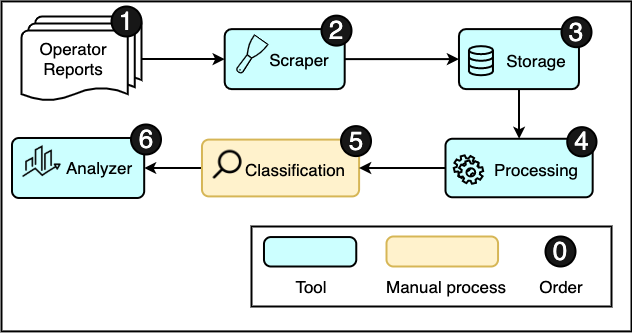
\includegraphics[scale=0.5]{diagrams/process.png}
  \caption{Data collection, extraction, and analysis process.}
  \label{fig:process diagram}
\end{figure}
Cloud providers self-report information about service availability and failures through public status pages.
We selected three of the largest worldwide cloud service providers: Amazon Web Services (AWS), Microsoft Azure, and Google Cloud Platform (GCP).
The whole workflow is shown in \autoref{fig:process diagram}.
We use data scraped from the providers' public status pages for self-reported failures \cite{awsFeed, gcpFeed, azureFeed} in the span of one year, Jan-Dec 2018.
The pages were scraped every six hours, to avoid burdening the page host with more frequent scrapes and potentially incurring penalties (step 2 in \autoref{fig:process diagram}).
The raw dataset is approximately 522 KiB in size; the cleaned and processed dataset is around 172 KiB.

We use Python 3.7.7, Pandas 1.0.3, NumPy 1.18.4, SciPy 1.4.1, and Pytz 2019.3 to process and analyze the extracted structured failure data.
We first deduplicate the data based on the service name, failure location, and event start time, selecting the events with the longest duration in cases where the other properties are equal (step 4 in \autoref{fig:process diagram}).
This removes 400 events in total: 137 from Azure, 127 from AWS, and 136 from GCP.
We convert all reported event start times to the timezones appropriate to the region specified for the outage.
We calculate the event duration in minutes based on the event start and end times.
We also compute the year the event took place, as well as the hour of the week (with hour 0 denoting midnight on Monday).
We then filter the data, selecting events that occurred in the 2018 calendar year.
This yields a grand total of 411 events: 139 from GCP, 144 from AWS, and 128 from Azure.

\subsection{Failure classification}
Service providers include in their reports a textual description of the outage.
The description does not follow a specific format or standard, and must thus be manually analyzed for each event.
We classify outages across several categories based on the description of the outage (step 5 in \autoref{fig:process diagram}).
The classification is partially based on that done by Gunawi et al. \cite{gunawi2016, gunawi2014}, but as many of the failure descriptions are terse and brief, we cannot capture as much detail in our classification.

The description provides information about the qualitative aspects of the outage.
We identify six such aspects: how many services were affected, the severity, the range, the users affected in the outage, the root cause of the outage, the duration of the outage.
An outage can affect one or multiple services; we assume that only one service is affected (namely, the reported service), unless the provider explicitly states otherwise in the description.
The severity can be strictly a visual error (i.e. performance is not affected, only visual feedback is incorrect), service performance degradation, or complete service unavailability.
The range of an outage can be limited to (in ascending order of geographical size) a single availability zone, a single region, or multiple regions.
As the range of a single availability zone only applies to AWS services, outages that occurred in a single availability zone (13 events) were merged with those occurring in a single region, to simplify analysis.
An outage can affect some users, or all users; this is understood in combination with the range of the outage (e.g. an outage may affect all users in a single region).
An event is assumed to affect all users of the service indiscriminately, unless the provider explicitly reports that only some users are affected.
The cause of an outage can be a code error, a side effect of maintenance, a configuration error, a network error, an external factor, increased load, or an unhealthy unit.
A ``unit'' is not necessarily a physical (i.e. hardware) unit, but can be a virtual node, a cluster, etc.

Some of these causes can be further separated into narrower categories.
A configuration error can stem from a direct change to a configuration file, or can happen as part of a deployment task.
A network error can indicate an internal API issue, or an internal network issue.
An external factor can be the environmental conditions in the datacenter (e.g. higher temperatures or humidity), a shock event (e.g. a thunderstorm), or an issue caused by a third party.

If one of the features is not stated in the description of a particular outage, we note that information about it was not provided for the outage.

  \section{Results \& analysis}
% "impact level": range + services
% "area of effect": range + users

\paragraph{Hourly and daily failure trends}
\begin{figure}[h]
  \centering
  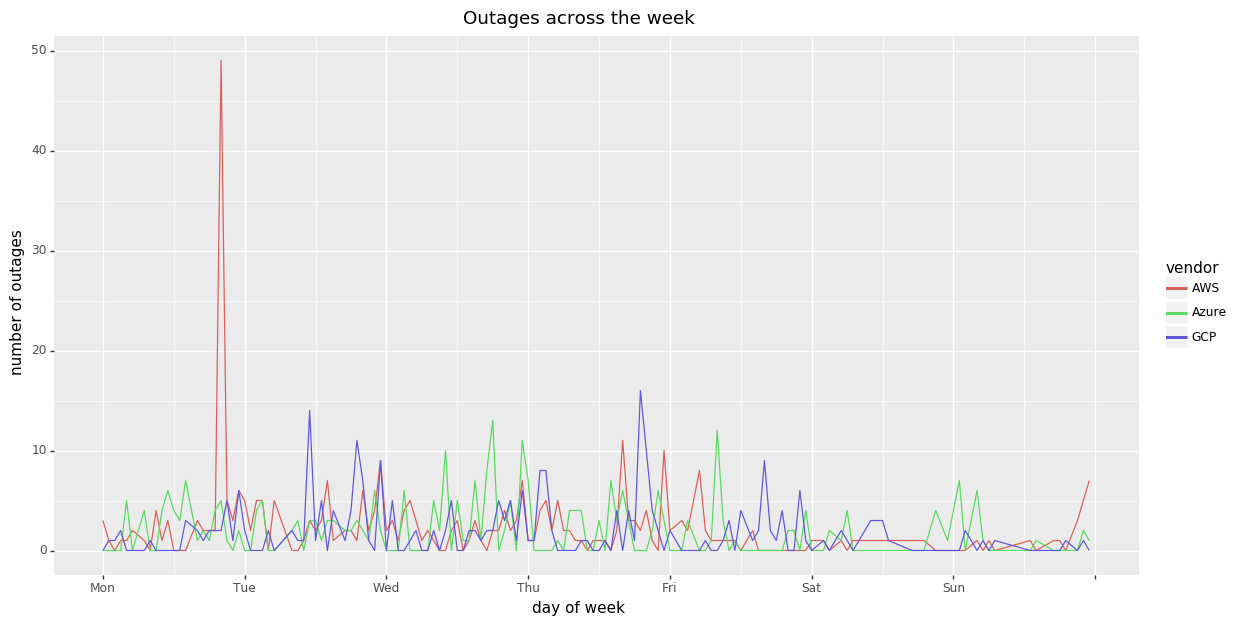
\includegraphics[scale=0.75]{outages-across-week.png}
  \caption{Distribution of outages across the week, separated by vendor.}
  \label{fig:outages across week}
\end{figure}

We first observe the distribution of outages across the week, this is shown in \autoref{fig:outages across week}.
GCP and AWS both display significant peaks at two points during the week: around the middle (Tuesday and Wednesday), and at the start of the weekend (Friday and Saturday).
AWS also shows an increase in outages in the afternoon/evening hours on Sunday.
The data provided by Azure does not indicate any clear trends.

\paragraph{Root causes of outages by impact level and vendor}
\begin{figure}
  \centering
  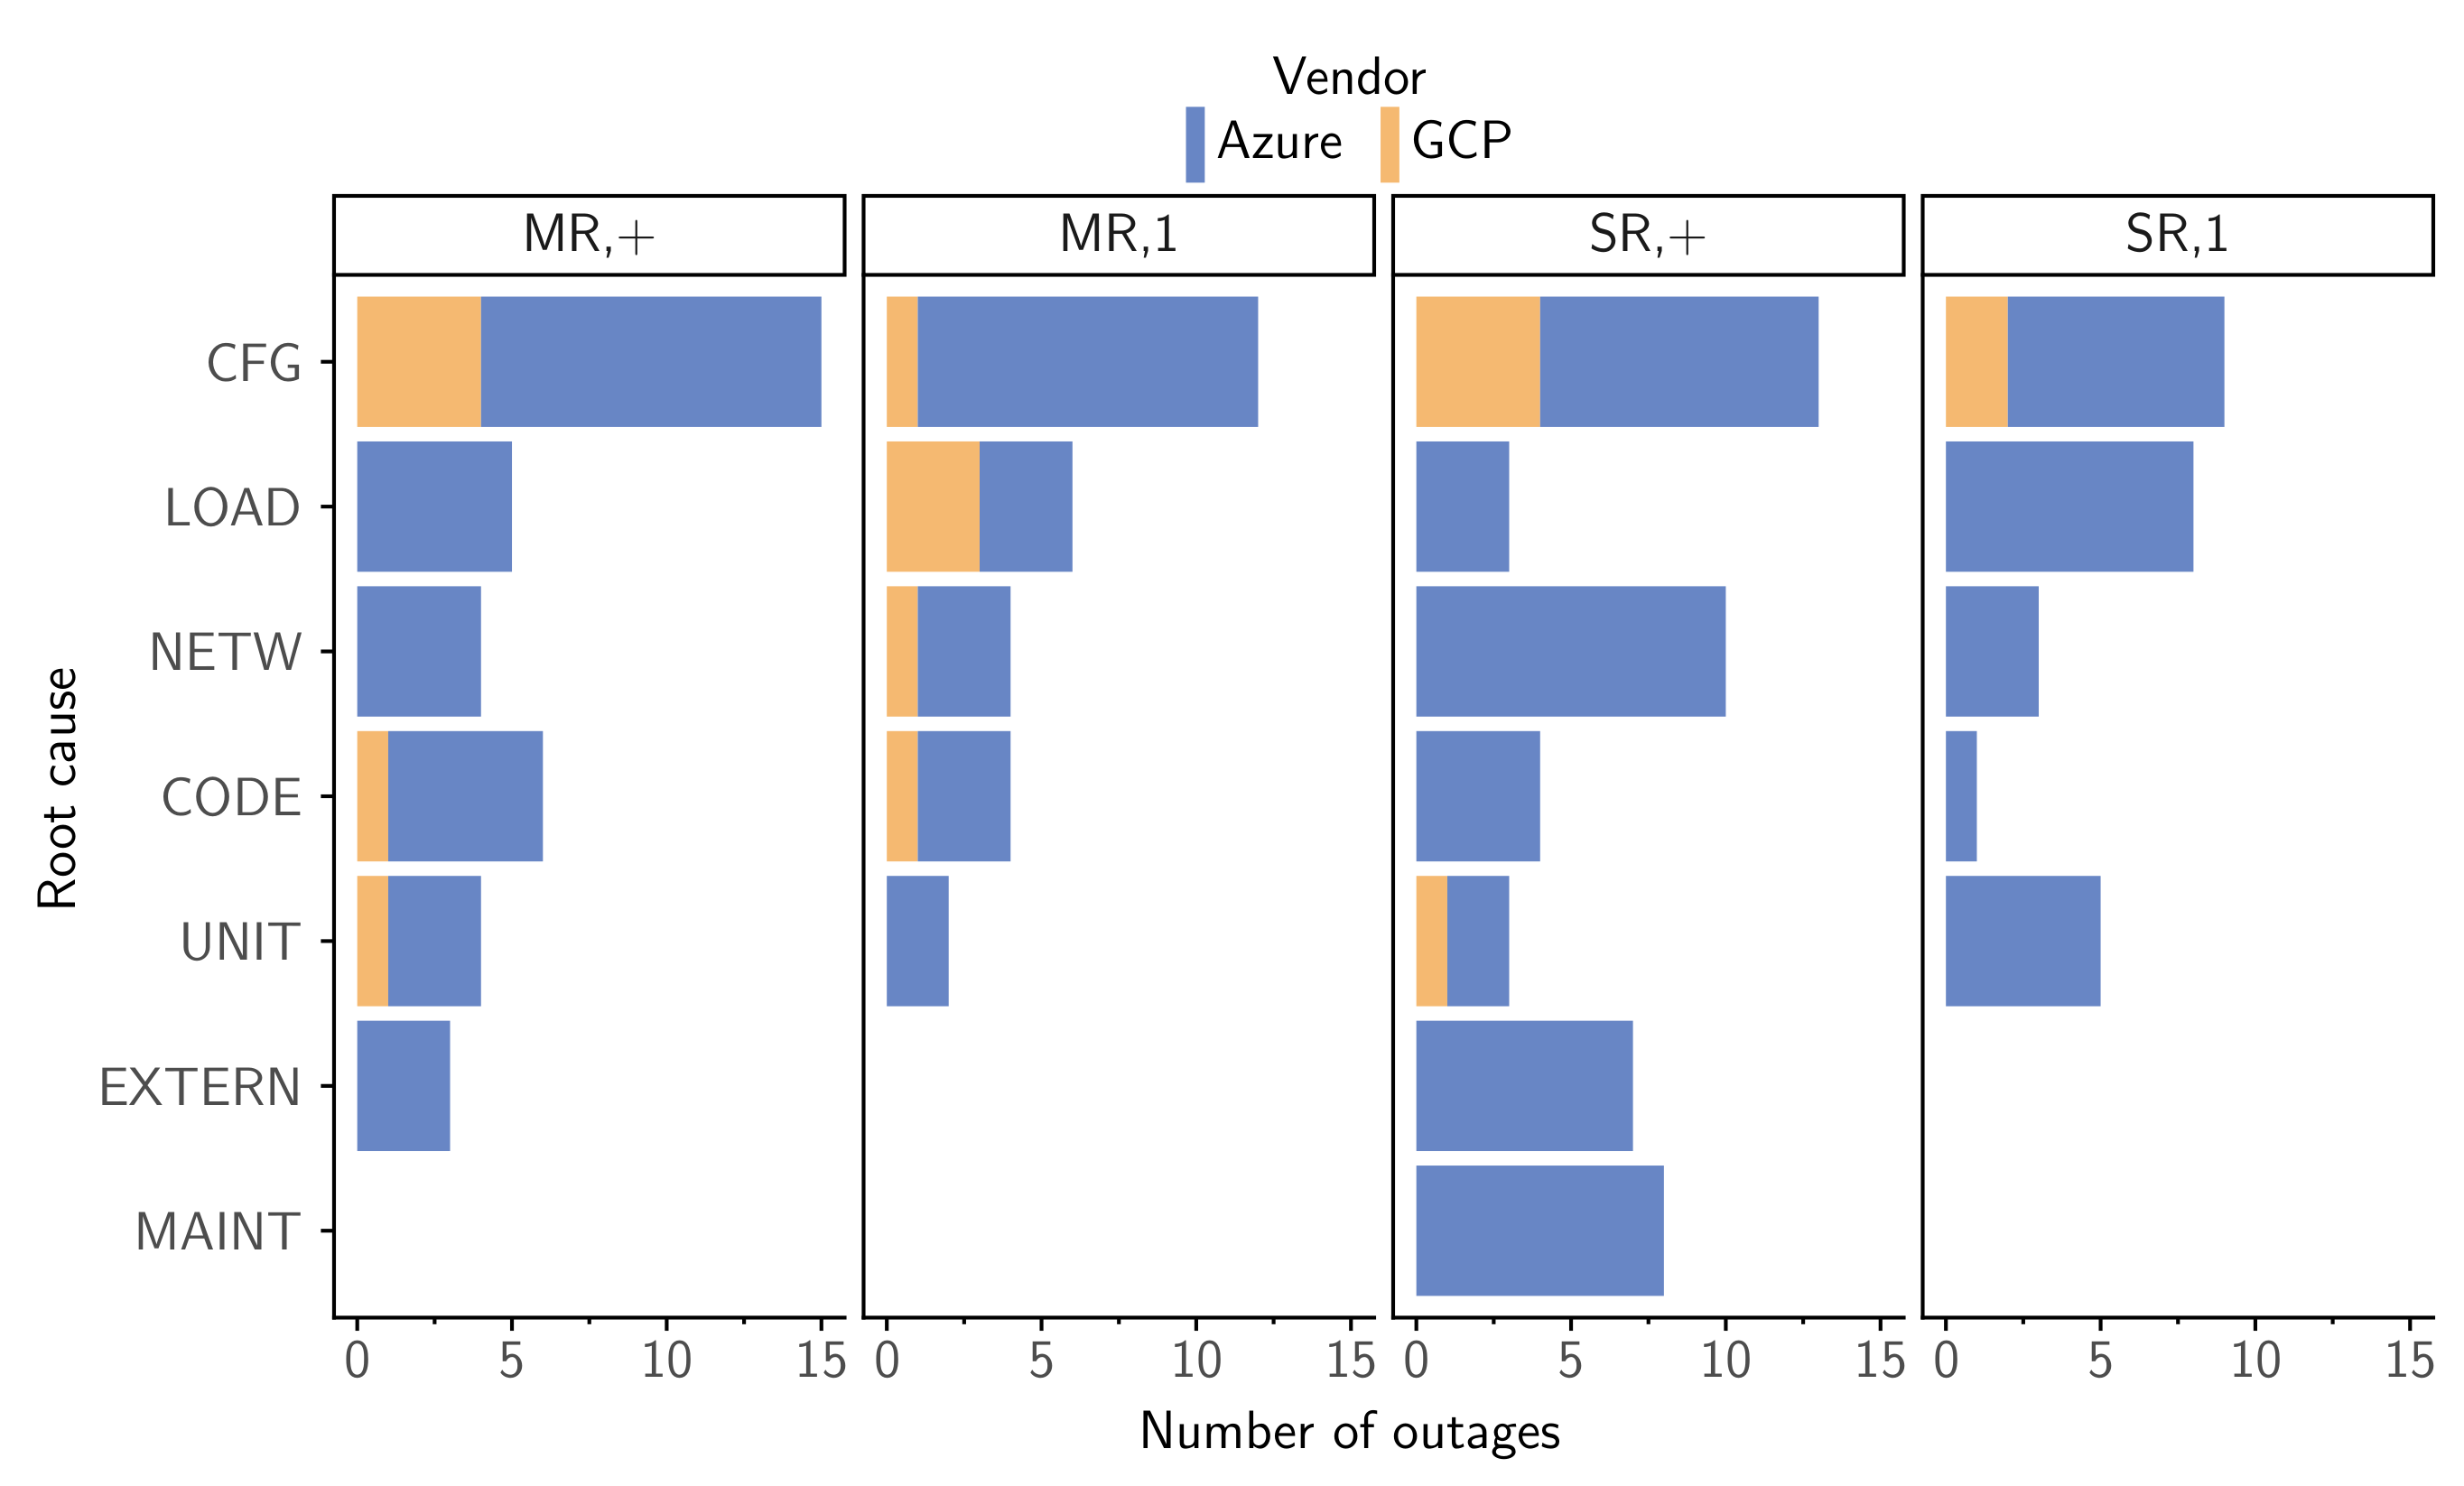
\includegraphics[scale=0.7]{root-causes-by-severity.png}
  \caption{Root causes of outages across varying impact levels, separated by vendor. (MR = multiple regions, SR = single region, 1 = one service, + = multiple services)}
  \label{fig:root causes by severity}
\end{figure}

We next analyse the distribution of outages across root causes and impact levels.
We identify seven classes of root causes: UNIT (individual nodes, instances, or clusters, not necessarily hardware), NETW (related to the internal or external network), MAINT (side effects caused by maintenance), LOAD (increased load on the service), EXTERN (external causes, i.e. environmental or third-party), CODE (code errors/bugs), and CFG (configuration errors).
We further separate the outages by vendor, indicated by the color of the bar in \autoref{fig:root causes by severity}.
We do not include AWS, as we do not have sufficient data regarding root causes from AWS (a cause was only specified for 2.1\% of AWS events).
Excluded from the plot are outages that did not provide a root cause (a total of \result{np-root-causes-by-severity-cause}), a range (\result{np-root-causes-by-severity-range}), or the number of affected services (\result{np-root-causes-by-severity-services}).

The majority of outages across all levels of impact are caused by configuration errors.
For multi-regional outages, the configuration category accounts for the majority by a wide margin.
On the other hand, for single-region outages, there are multiple leading causes: apart from configuration errors, outages affecting one service are also caused by increased load and failing instances, and those affecting more than one service are also caused by network errors and maintenance side effects.

\paragraph{Failure distribution across the week, separated by root cause}
\begin{figure}
  \centering
  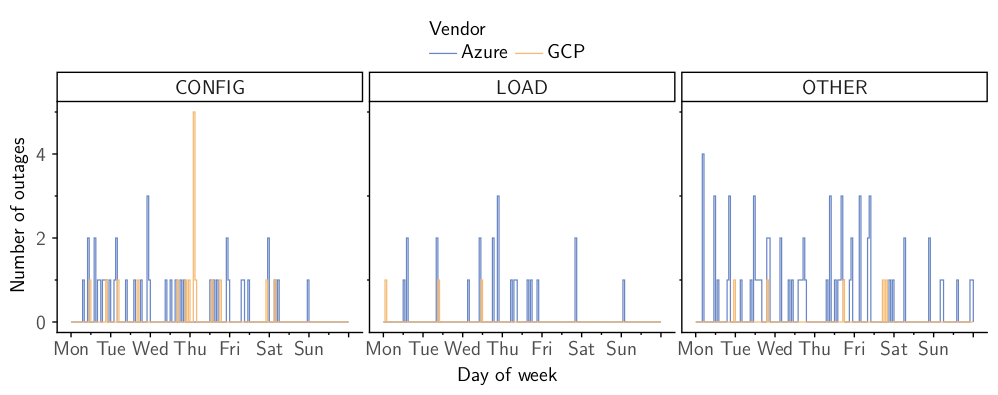
\includegraphics[scale=0.7]{causes-across-week.png}
  \caption{Outages across the week, separated by root cause and vendor. (CONFIG = configuration error, LOAD = increased load, OTHER = other)}
  \label{fig:causes across week}
\end{figure}

We analyze the frequency of root causes at various points in the week, separated by vendor.
We exclude AWS outages, due to a lack of specified root causes.
Outages from other providers that did not state a root cause are also excluded (\result{np-causes-across-week-cause}).
From \autoref{fig:causes across week}, it seems that load-related outages tend to happen starting between midday on Wednesday and Thursday evening, with smaller peaks during the night on other days.
Most outages caused by misconfiguration happen in the first half of the week, from mid-Monday until midnight on Thursday.
This could perhaps be because large code changes are usually introduced during the first few days of the week.
The major peaks for these outages generally occur around midnight.
The reason for this could be that deployments happen during the night, when it is likely that fewer customers will be using the service; as Langford et al. found, there is a significant difference in traffic during the day and during the night \cite{langford2012}.
It could also be that changes are deployed during the day, but there is a delay before bugs appear.
Outages related to other root causes generally occur during the weekdays, and there are only a few peaks during the weekend.
It is important to note here that this is a relatively small dataset, and the trends observed in \autoref{fig:causes across week} could change if more data becomes available.

\paragraph{Root causes of outages, separated by duration and vendor}
\begin{figure}
  \centering
  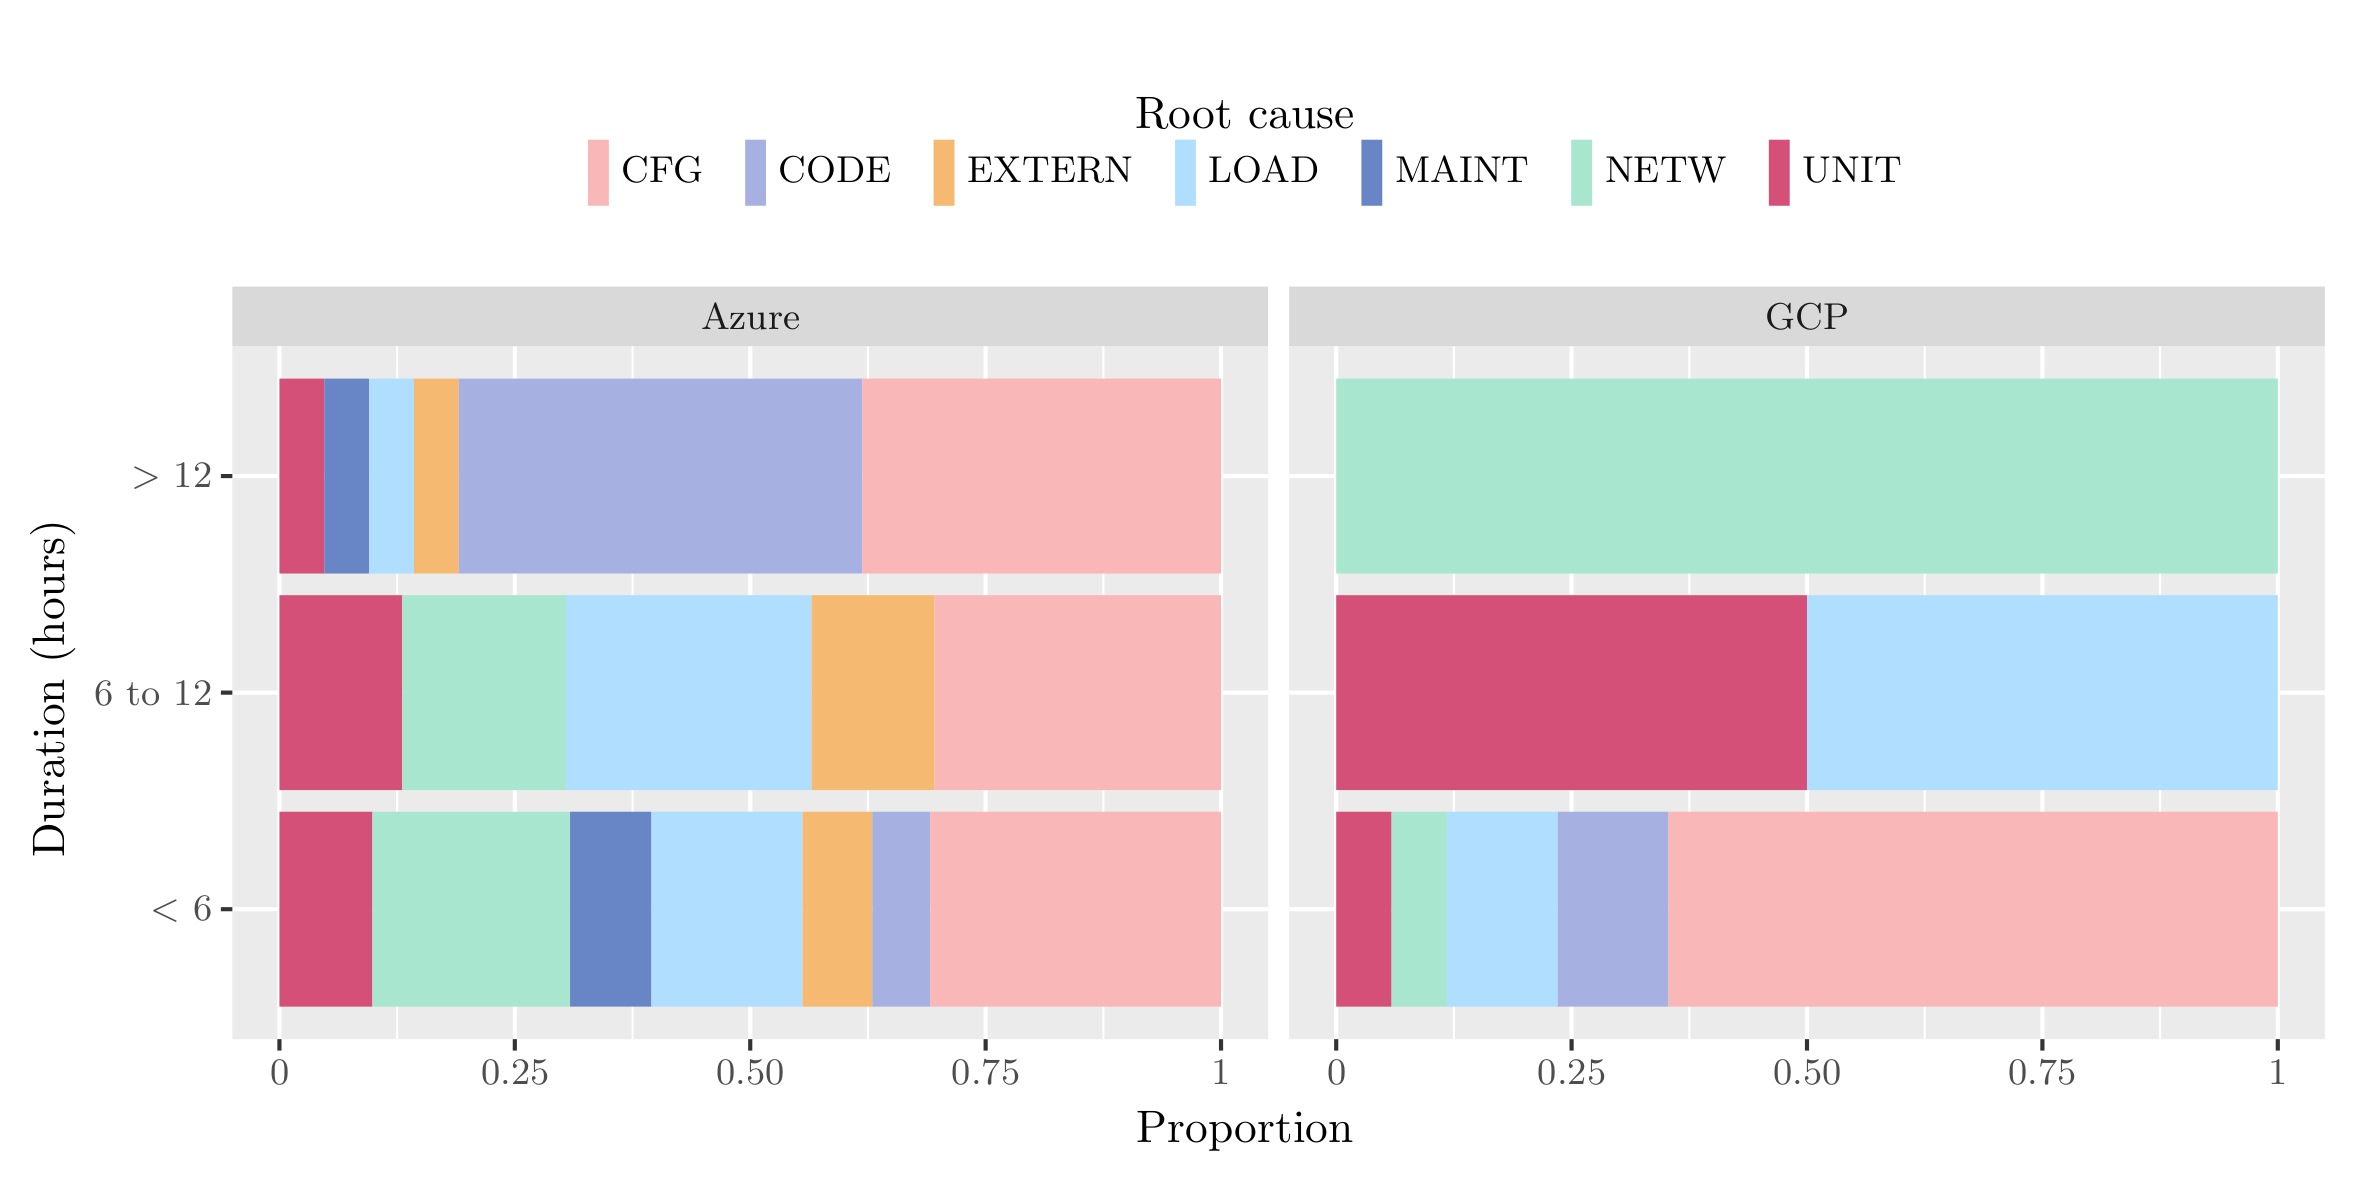
\includegraphics[scale=0.7]{causes-vs-duration-hr-ranges.png}
  \caption{Root causes of outages, separated by duration and vendor. (CFG = configuration error, CODE = code error, EXTERN = external, LOAD = increased load, MAINT = maintenance, NETW = network, UNIT = failing unit (physical/virtual))}
  \label{fig:causes vs duration ranges}
\end{figure}

We separate the outages by duration, in three categories: short (outages lasting less than six hours, `$<$ 6'), medium (six to twelve hours, `6 to 12'), and long (more than twelve hours, `$>$ 12').
The outages are grouped by duration and vendor, such that the horizontal axis shows the proportion of outages for a specific duration category and vendor.
We do not plot outages that did not specify a root cause (\result{np-causes-vs-duration-hr-ranges-cause}).
All AWS outages that specified a cause were shorter than six hours, and were caused by external events (e.g. third party or environment).
However, as discussed above, only three AWS outages specified a cause, so AWS is not included in \autoref{fig:causes vs duration ranges}.
Azure services have more diverse outage causes than GCP services.
All outages of GCP services that lasted longer than twelve hours were caused by network errors; in contrast, network errors did not play a role in these types of outages for Azure services.
The longest outages of Azure services were caused in approximately equal parts by code and configuration errors.
Configuration errors were a common cause of Azure outages for all three duration categories, while only the shortest GCP outages (shorter than six hours) had configuration errors as a cause.
For both GCP and Azure, increased load was a main factor in the short- and medium-duration outages.
For GCP, there were more medium-duration outages caused by increased load than short-duration outages; for Azure services, the proportion is approximately the same.
GCP also had failing computational units as a major cause for medium-duration outages; this was not as prominent for Azure services, where failing units accounted for approximately the same proportion of short-duration outages as for medium-duration outages.

\paragraph{Root causes of outages, separated by area of effect}
\begin{figure}
  \centering
  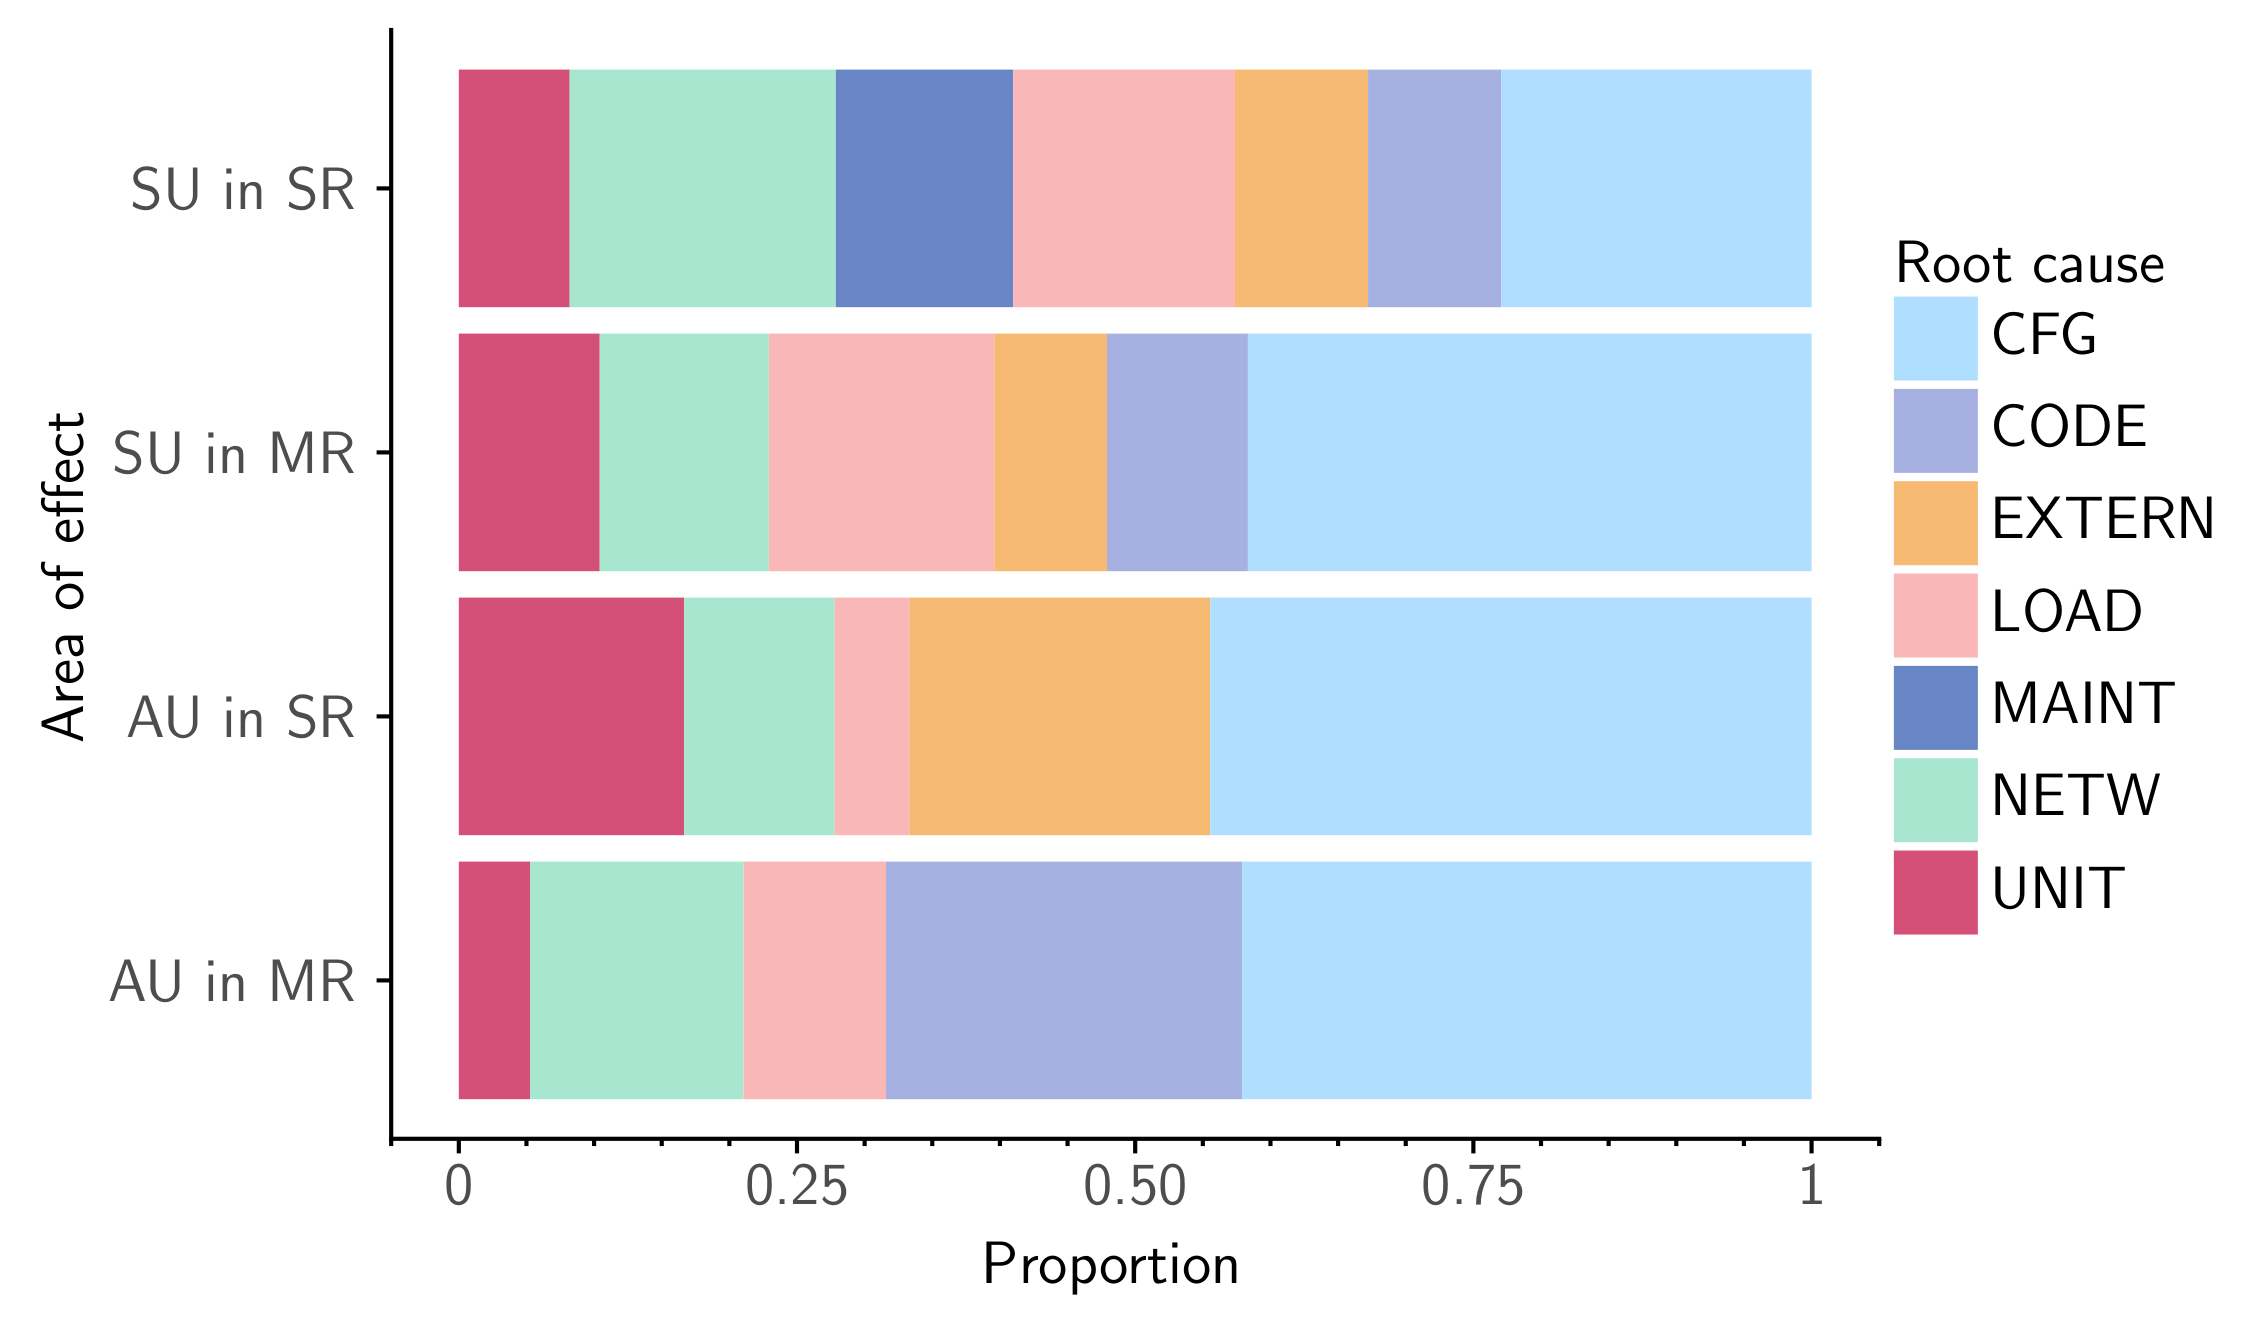
\includegraphics[scale=0.7]{range-users-vs-root-cause.png}
  \caption{Root causes of outages at various areas of effect. (SU = some users, AU = all users, SR = single region, MR = multiple regions)}
  \label{fig:causes vs aoes}
\end{figure}

We also analyze the root causes of outages, separated by the area of effect.
Here we exclude those events that did not provide a cause (\result{np-range-users-vs-root-cause-cause}), a range (\result{np-range-users-vs-root-cause-range}), or the affected users (\result{np-range-users-vs-root-cause-users}).
From \autoref{fig:causes vs aoes}, we conclude that configuration errors account for the majority of outages with the widest area of effect (all users in multiple regions).
The second main cause of such outages are code errors, which interestingly do not play a major role in single-region outages, and do not appear as a cause of single-region outages affecting all users.
Failing instances are mainly a cause of single-region outages, more so for outages that affect all users -- this is probably due to the fact that individual instances, nodes, or clusters are localised in a single region \cite{awsRegionDocs}.
From the available data, it seems that outages caused as a maintenance side effect only affect some users of the service, mostly in a single region.
It also appears that outages caused by increased load more commonly affect only some users in a given range.
The majority of outages caused by network issues affect some users in a single region, though they also play a somewhat significant role in the other area of effect categories (accounting for around 10\% of the outages in each category).

\paragraph{Severity and duration of failures by the area of effect}
\begin{figure}
  \centering
  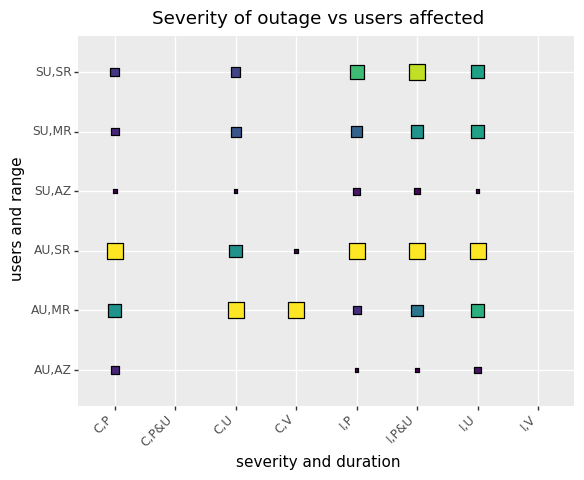
\includegraphics[scale=0.7]{severity-vs-users-affected.png}
  \caption{Severity of an outage and the users affected by the outage. (SU = some users, AU = all users, Cont = continuous, Interm = intermittent, Perf = performance degradation, Unavail = unavailable, Vis = visual)}
  \label{fig:severity vs users}
\end{figure}

Next, we consider the severity and duration of an outage, depending on its area of effect.
We exclude events that did not state the affected users (\result{np-severity-vs-users-affected-users}), range (\result{np-severity-vs-users-affected-range}), severity (\result{np-severity-vs-users-affected-severity}), or duration (\result{np-severity-vs-users-affected-duration}).
The first immediate finding from \autoref{fig:severity vs users} is that the majority of outages result in one or more services becoming intermittently unavailable.
For outages affecting all users, in a single region or in multiple regions, there is a higher proportion of outages that cause a service to be intermittently degraded or unavailable than for outages affecting some users.
Furthermore, the majority of outages that resulted in a service being continuously unavailable (for some period of time) affected all users in multiple regions.
When the performance of one or more services is degraded, it generally happens for a continuous period of time.

\paragraph{Outages separated by area of effect and vendor}
\begin{figure}
  \centering
  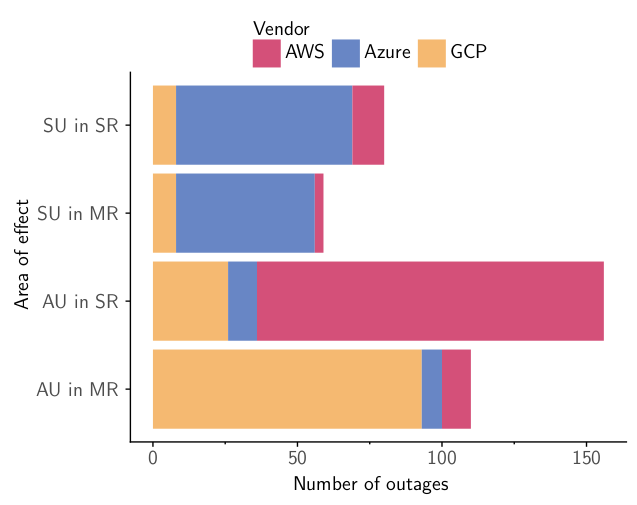
\includegraphics[scale=0.7]{users-affected-by-vendor.png}
  \caption{Area of effect of outages by vendor. (AU = all users, SU = some users, SR = single region, MR = multiple regions)}
  \label{fig:aoe by vendor}
\end{figure}

We analyse the distribution of outages per vendor, in figure \autoref{fig:aoe by vendor}.
We do not include events that are missing information about the users (\result{np-users-affected-by-vendor-users}) or the area of effect (\result{np-users-affected-by-vendor-range}).
We observe that the range of the majority of outages depends on the vendor.
The majority of GCP outages affect all users in multiple regions, while the majority of AWS outages affect all users in a single region.
For Azure services, the outages mostly affect some users, with an approximately equal distribution between a single region and multiple regions.

\clearpage

\paragraph{Correlation analysis (Cram\'{e}r's V)}
\begin{figure}
  \centering
  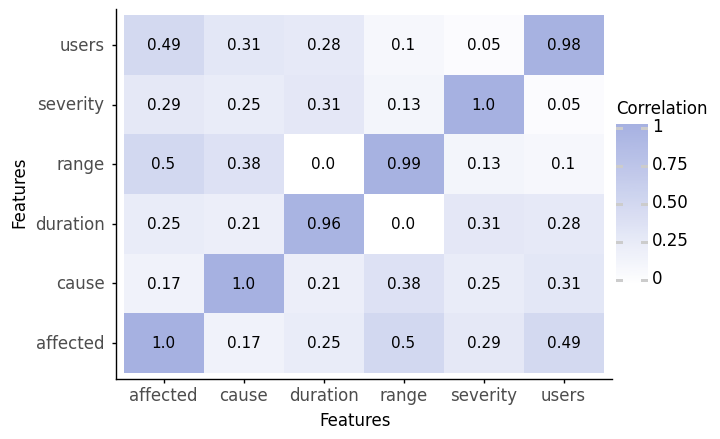
\includegraphics[scale=0.7]{cramers-v.png}
  \caption{Correlation matrix (Cram\'{e}r's V)}
  \label{fig:cramers v}
\end{figure}

Finally, we conduct correlation analysis on the various features of the data.
The first statistic we consider is Cram\'{e}r's V (also known as Cram\'{e}r's phi coefficient, written as $\phi_c$), which measures association between two variables.
It extends the phi coefficient to contingency tables larger than $2 \times 2$, and results in a value between 0 and 1, with 0 indicating no correlation.
Cram\'{e}r's V is computed as:

$$
V = \sqrt{\frac{\chi^2}{n \times \min{(k-1, r-1)}}}
$$

where $r$ is the number of rows and $k$ the number of columns in the contingency table, $n$ is the number of observations, and $\chi^2$ is derived from Pearson's chi-squared test \cite{holmes1998}.

Applying the measure to the dataset, we obtain a correlation matrix shown in \autoref{fig:cramers v}.
We observe that there is no strong correlation between any of the features.
Relative to the other values in the matrix, the component affected in the outage seems to be moderately correlated with the range of the outage (0.5), and with the users affected in the outage (0.49).
There may also be a slight correlation between the cause of the outage and the range of the outage (0.38), as well as with the users affected in the outage (0.31).
However, since the values are low, these results are inconclusive.

\paragraph{Association analysis with the uncertainty coefficient (Theil's U)}
\begin{figure}
  \centering
  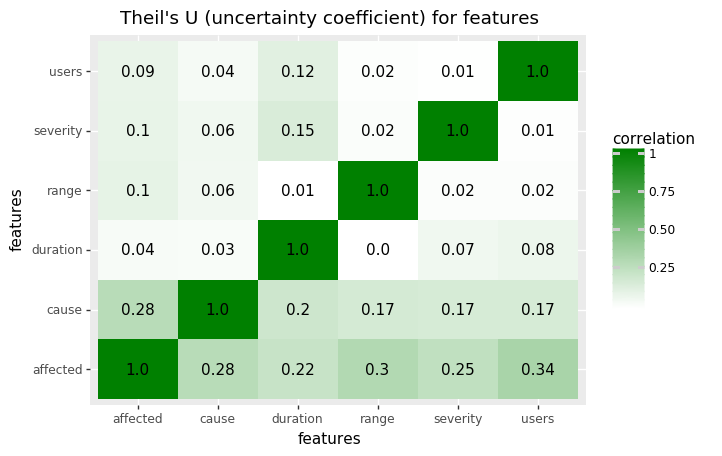
\includegraphics[scale=0.7]{theils-u.png}
  \caption{Uncertainty coefficient matrix (Theil's U)}
  \label{fig:theils u}
\end{figure}

We calculate uncertainty coefficients, also known as Theil's U, for the features of the data; this is shown in a matrix in \autoref{fig:theils u}.
The uncertainty coefficient of $y$ with respect to $x$, written as $U(y|x)$, shows how much information $x$ provides about $y$, and is a value between 0 and 1.
A value of 0 indicates that $x$ gives no information about $y$, and a value of 1 that knowledge of $x$ completely predicts $y$.
Computing Theil's U clarifies the associations seen from Cram\'{e}r's V: the symmetry of Cram\'{e}r's V does not necessarily hold for the actual correlations.
The uncertainty coefficient provides more information about the true relations between the different features \cite{zychlinski2018}.

$U(y|x)$ is computed as:

$$
U(y|x) = \frac{H(y) - H(y|x)}{H(y)}
$$

where $H$ is entropy of a single distribution, and $H(y|x)$ is the entropy of $y$ conditional on $x$ \cite{press2007}.

The results in \autoref{fig:theils u} show no clear association, as the coefficients are low.
However, the users affected in the outage could determine the affected component (0.34) and range of the outage (0.3).
This seems to support the findings from \autoref{fig:cramers v}.
Similarly, the affected component could determine the cause of the outage (0.28).

  \section{Threats to Validity}
Having presented the results and analysis, this section discusses the main limitations of the study.

\paragraph{1. Manual classification of data points.}
Due to the lack of structure or standard format among the failure descriptions, all events had to be classified manually across different categories (step 5 in \autoref{fig:process diagram}).
Though the classification was conducted diligently and checked multiple times, such a process is vulnerable to human error.
Furthermore, by relying on our interpretation of the descriptions for classification, we introduce an element of subjectivity in the dataset.
It is possible that some events are misclassified, which would negatively affect the validity of our results.
Unfortunately, because of the aforementioned lack of structure in the reports and insufficient tools for analysis of such data, this is currently unavoidable.

\paragraph{2. Lack of available data.}
In our analysis, we use a dataset with a relatively small amount of events.
To draw more significant and valid conclusions, a much larger dataset would be needed.
As no such public repository of data is currently available, we do not have a way to obtain these data.
Moreover, for some analyses, we exclude a few data points due to insufficient information.
Such selective cleaning may lead to unintended consequences or biases in our results.
Finally, as information about failures could be damaging to cloud providers, the self-reporting process could result in bias in the data itself.

\paragraph{3. Heuristic processing errors.}
For AWS and Azure failures, we extract the event start and end time from textual descriptions.
We use heuristic methods based on sentence structures.
Despite taking the utmost care, there is a non-zero possibility that we might have missed or wrongly attributed certain failures.

  \section{Related work}\label{sec:related work}
Having presented and discussed our results, we examine previous work done in the field.

One similar study is that of Gunawi et al. \cite{gunawi2016}, who analyze the availability of popular cloud services during a time period of seven years.
They examine services for online chat (e.g. WhatsApp), e-commerce (e.g. Amazon.com), email (e.g. GMail), SaaS (e.g. Salesforce), video streaming (e.g. Netflix), and others.
They collect data from news headlines, and from the providers' public post-mortem reports (published after the failure event).
Similarly to our study, they manually tag the outages with metadata.
This metadata describes the root causes, impacts, fixes, downtime, type (planned or unplanned), and service scope of each outage.
Due to the nature of their dataset, they are able to extract more detail in some metadata categories, such as root causes.
They find that almost 50\% of the services they analyze experience an average of three or more outages per year, and 25 services do not reach 99.9\% uptime.
These outages do not decrease as the service matures; rather, as a service matures, it becomes more popular, and thus need to handle more users and increases in complexity.
Perhaps complementary to our findings regarding root causes of outages, fixing software is a major fix procedure category in their results, accounting for 22\% of all outages.
Their analysis of root causes shows that to ensure that cloud services do not have a single point of failure, perfection is required along the whole failure recovery chain.
They also conduct a detailed analysis of root causes of outages.

Another related study focuses on popular cloud systems, particularly on those generally not seen by end users \cite{gunawi2014}.
These include Hadoop MapReduce, Hadoop File System, HBase, Cassandra, ZooKeeper, and Flume.
The aim of the study is to characterise the bugs present in cloud systems.
Gunawi et al. collect data from issue repositories maintained by the development projects of the aforementioned systems.
The issues are generally submitted by the developer or user community of the system.
The authors select issues submitted over a period of three years, and analyze patches and developer responses for the issues.
They conduct a manual classification of the issues for each service, applying metadata labels related to the aspect of the issue (reliability, performance, availability, etc.), hardware type, failure mode (stop, corrupt, or ``limp''), and bug scope (single machine, multiple machines, or a whole cluster).
They find that 8\% of bugs are unique to cloud systems, and that even though there are software measures in place, 13\% of issues are still caused by hardware failures.
Their results also suggest that cascades of failures can occur in subtle ways from a ``killer bug'', which is perhaps similar to how failures can cascade across services in our analysis.
Finally, the largest category of software bugs in their results consists of those that are logic-specific, which complements our findings.

There have also been other studies of failures in the cloud, with various aims.
Some have focused on failure analysis in the area of high-performance computing (HPC).
The majority of high-performance computing studies use data from providers, and conduct an analysis of large-scale production systems such as the Google Cloud cluster or the Los Alamos National Lab, or supercomputers such as the Titan or Eos \cite{chen2014, elsayed2017, liang2006, zheng2011, kavulya2010, gupta2015, gupta2017, di2019, elsayed2013, martino2014, schroeder2010, javadi2013, schroeder2007}.
The data used in these studies most commonly comes from traces and reliability-availability-stability (RAS) logs, with some studies using job logs and system logs; one study conducts a combined analysis of RAS logs and job logs \cite{zheng2011}.
There is also one analysis of HPC system failures with user-reported data \cite{gray1986}.
Next, perhaps closer in subject to our work, there have been a number of studies analyzing provider data for failures in large-scale services, such as storage systems and cloud platforms \cite{oppenheimer2003, ford2010, schroeder2007, javadi2013, garraghan2014, yalagandula2004, li2013, zhou2015}.
Those that study more customer-facing services such as Apache Cassandra, Amazon S3, or MySQL generally utilize user-reported data \cite{frattini2013, yuan2014, palankar2008, fonseca2010, fonseca2010, benson2010, jiang2008, yin2011}.
Compared to these studies, our work contributes an analysis of customer-facing services using data from providers; in particular, the data they report publicly, as opposed to data from internal error tracking databases or reports.
Some studies synthesize data from both providers and customers \cite{ostermann2008, sahoo2010}.
Finally, other analyses investigated network failures using provider data \cite{gill2011, banerjee2015, turner2010}, and virtual/physical machine failures using either provider data \cite{vishwanath2010, nightingale2011, rosa2015} or a combination of provider and user data \cite{birke2014}.

  \section{Conclusion}
Cloud services run many of the modern applications we use today, and are expected to be constantly available.
This is not always the case, as services outages happen relatively frequently.
When a service goes down, other services that depend on it may also fail.
Therefore, prevention is key, and understanding how these outages happen is the first step towards preventing them.
In this paper, we have conducted a study of public cloud provider reports of outages during the 2018 calendar year.
We developed a framework for classifying and analyzing these reports, and used it to examine the collected data.
We identified the challenges associated with the gathering and analysis of failure data, and extracted patterns relating to the failure of cloud services.
Some of the data we generated and analyzed in this study has been used for a section of a paper submitted to a top conference.

Future work in this area could address some of the limitations and concerns discussed in \autoref{sec:threats to validity}.
In particular, the classification process could be improved, perhaps via language processing algorithms.
This would eliminate the need to classify events manually, reducing the probability of erroneous classification.
Furthermore, data limitations could be addressed by conducting a synthesis of all data from various sources, such as news reports, provider reports, and user reports.
Data from multiple sources for a particular outage could be correlated using timestamps, or other identifying features.
This would provide a more objective view of the data, and would result in a much larger dataset.


  \printbibliography

  \appendix
  \section{Problem statement}


  \section{Self-reflection}
This was the first opportunity I had to conduct a `proper' research project, and as such benefited me greatly.
I learned how to clean a large dataset, and how to conduct a scientific analysis of that dataset.
I also learned how to compile the process and results into a research paper, and how to look for and analyse related articles.
The possibility of contributing to a paper submitted to a top conference was a great motivator.
Overall, the project helped me develop into a more independent researcher.

The largest period of time was spent on the preparation of the dataset; that is, on cleaning and labelling the dataset for analysis.
The manual classification of events was especially time-consuming.
The second longest amount of time was spent on analysis of data, particularly on selecting the best aspects to analyze and creating good visualisations of the results.
The rest of the time was spent on researching, and on writing the report.

\end{document}
